\documentclass{standalone}
\usepackage{tikz}
\usepackage{pgfplots}
\pgfplotsset{compat=1.16}

\begin{document}

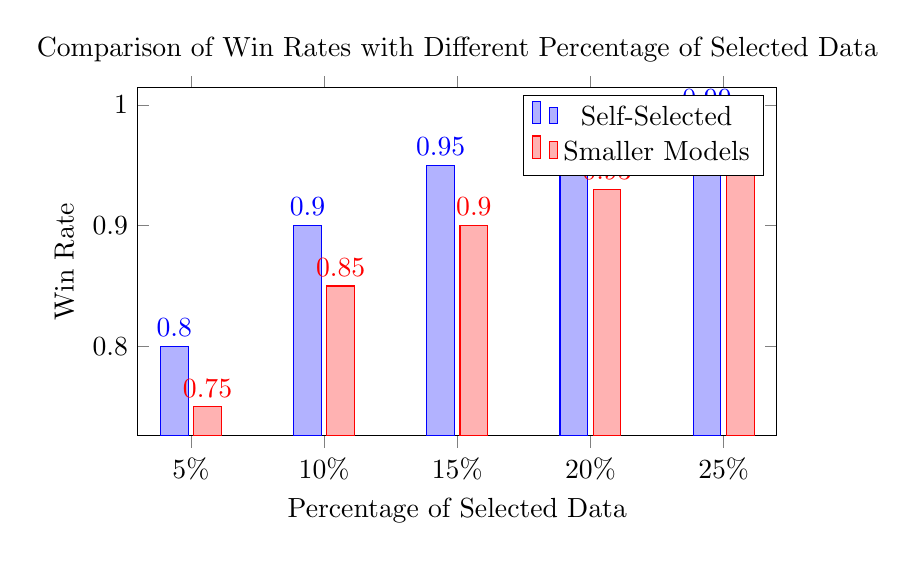
\begin{tikzpicture}
    \begin{axis}[
        ybar,
        symbolic x coords={5\%, 10\%, 15\%, 20\%, 25\%},
        xtick=data,
        nodes near coords,
        ylabel={Win Rate},
        xlabel={Percentage of Selected Data},
        title={Comparison of Win Rates with Different Percentage of Selected Data},
        width=0.8\textwidth,
        height=6cm
    ]
        \addplot coordinates {(5\%, 0.8) (10\%, 0.9) (15\%, 0.95) (20\%, 0.98) (25\%, 0.99)};
        \addplot coordinates {(5\%, 0.75) (10\%, 0.85) (15\%, 0.9) (20\%, 0.93) (25\%, 0.95)};
        \legend{Self-Selected, Smaller Models}
    \end{axis}
\end{tikzpicture}

\end{document}